% +--------------------------------------------------------------------+
% | Your paper should contain the following sections, except where     |
% | indicated as optional, in the order shown.  Also, all headings     |
% | shown with an asterisk (*) must be centered and in uppercase       |
% | letters:                                                           |
% |                                                                    |
% | Abstract Title Page (doctoral dissertations only)                  |
% | ABSTRACT* (doctoral dissertations only)                            |
% | Title Page                                                         |
% | Copyright Page (Optional - only needed if copyrighting)            |
% | ABSTRACT *                                                         |
% | TABLE OF CONTENTS *                                                |
% | LIST OF FIGURES *                                                  |
% | LIST OF TABLES*                                                    |
% | ACKNOWLEDGMENTS* (Optional)                                        |
% | DEDICATION * (Optional)                                            |
% | PREFACE * (Optional)                                               |
% | Individual Chapters                                                |
% | References and/or bibliography                                     |
% | Appendices (as needed)                                             |
% +--------------------------------------------------------------------+

% +--------------------------------------------------------------------+
% | The LaTex keyword \documentclass selects a particular class to     |
% | associate with the document.  The current documentclass            |
% | {class_diss} generates a Table of Contents that has leading dots   |
% | only on chapter subheadings.  If you prefer a Table of Contents    |
% | that has leading dots for all entries, replace {class_diss}        |
% | with {Mydiss} in the command below.                                |
% |                                                                    |
% +--------------------------------------------------------------------+

\documentclass[final,12pt,oneside]{class_diss}

\usepackage[utf8]{inputenc}
\usepackage[T1]{fontenc}
\usepackage[USenglish,spanish]{babel}

%\usepackage{     caption2} % Customize captions a bit more
\usepackage{      amsmath} % American Mathematics Society standards
%\usepackage{      wrapfig} % Wraps text around a figure or table
\usepackage{     graphicx} % Extended graphics package.
%\usepackage{     fancyhdr} % Efficiently handles headers and footers
%\usepackage{       braket} % Bra-Ket notation package
%\usepackage{     mathrsfs} % Specialized Math fonts (Hamiltonian, etc.)
%\usepackage{boxedminipage} % Boxed text can be produced
%\usepackage{     setspace} % Controls line spacing via \begin{space}
\usepackage{adjustbox}
\usepackage{tabularx}
\usepackage[vlined,linesnumbered,noresetcount]{algorithm2e}

\usepackage{amsxtra}
\usepackage{amssymb}
\usepackage{amsthm}
\usepackage{latexsym}

\usepackage[usenames]{color}
\definecolor{  Pink}{rgb}{1.0, 0.5, 0.5}
\definecolor{Maroon}{rgb}{0.8, 0.0, 0.0}

% +--------------------------------------------------------------------+
% | In the commands below, we use the 'natbib' package, and specify    |
% | the 'sort&compress' option, which condenses                        |
% | citations from (1,2,3,5,9,10,11) to (1-3,5,9-11).  The 'bibpunct'  |
% | option selects various parameters for how the citation will be     |
% | displayed.  In this case, only the comma (separation between       |
% | citations) and the 's' (superscript) arguments are chosen.  The    |
% | other curly braces deal with how to 'wrap' the citation (using     |
% | parentheses, brackets, etc.) and are not needed for the chosen     |
% | style.                                                             |
% +--------------------------------------------------------------------+

\usepackage[sort&compress,numbers,square]{natbib}
\bibpunct[; ]{[}{]}{,}{n}{}{}
\usepackage{hypernat}

\usepackage[pdftex, plainpages=false, pdfpagelabels]{hyperref}

\hypersetup{
   linktocpage=true,
   colorlinks=true,
   bookmarks=true,
   citecolor=blue,
   urlcolor=red,
   linkcolor=Maroon,
   citebordercolor={1 0 0},
   urlbordercolor={1 0 0},
   linkbordercolor={.7 .8 .8},
   breaklinks=true,
   pdfpagelabels=true,
}

\topmargin      = -0.56in
\textheight     =  8.60in
\textwidth      =  6.46in
\oddsidemargin  =  0.02in

\newcommand{\todo}[1]{{\color{red}\bf borja: #1}}
\begin{document}
   \setcounter{page}{-1}

   \newpage
\thispagestyle{empty}
\begin{center}
   \vspace{1cm}
   {\Large A FAST IMPLEMENTATION OF PARALLEL SNAPSHOT ISOLATION}\\
   \vspace{1cm}
   {\large Borja Arnau de Régil Basáñez}\\
   \vspace{0.85cm}
   
\includegraphics[height=2.5in]{figures/escudo.png}

   \vspace{0.85cm}
   Trabajo de Fin de Grado del Grado en Ingeniería\\
   Informática\\

   \vspace{0.2cm}
   Facultad de Informática,\\
   Universidad Complutense de Madrid \\

   \vspace{1cm}
   Junio 2020
\end{center}

{\raggedleft
   \vspace{2cm}
   Director: Maria Victoria López López\\
   Co-directores: Alexey Gotsman \& Manuel Bravo\\
}

   \pdfbookmark[0]{Portada}{PDFPortadaPage}

% +--------------------------------------------------------------------+
% | On the line below, set the number to represent the page number of
% | the Table of Contents page.  For example, if the Table of Contents
% | page is the 8th page of your document, enter 8 in the brackets.  This
% | number may vary, depending on the length of your abstract.
% |
% | Numbers do not appear on the title and abstract pages, but they are
% | included in the page count.  The Table of Contents page is the
% | first page on which page numbers are displayed.
% +--------------------------------------------------------------------+

   \pagenumbering{roman}
   \setcounter{page}{-1}
   \phantomsection
   \selectlanguage{USenglish}
   \tableofcontents
   %\listoffigures
   %\listoftables

   \newpage

\begin{center}
{\bf \Huge Acknowledgements}
\end{center}

\vspace{1cm}

To my advisors Maria Victoria López López at Universidad Complutense de Madrid, and Alexey Gotsman and Manuel Bravo at the IMDEA Software Institute, for their guidance and support, and for giving me the opportunity to work along them.\\

I also thank Christopher Meiklejohn, who allowed me to work with him, and gave me the opportunity to discover the IMDEA Software Institute. To my colleagues at IMDEA, for giving advice and offering a helping hand.\\

Finally, to my girlfriend Paula, and my family, for their love, patience and support.\\

   \phantomsection
   \addcontentsline{toc}{chapter}{Acknowledgements}

   \newpage
\begin{center}
    {\bf \Huge Dedication}
\end{center}
\vspace{1cm}
\setlength{\baselineskip}{0.8cm}

Texto...
   \phantomsection
   \addcontentsline{toc}{chapter}{Dedication}

   \newpage

\begin{center}
{\bf \Huge Abstract}
\end{center}

\vspace{1cm}

\todo{Keep this paragraph, merge the next two into a single one, to say that both PSI and NMSI help. However, sometimes the programmer wants stronger consistency (SI). In this work, we propose a variant of PSI that allows stronger consistency, while still being ``fast''.}

Most distributed database systems use weak consistency protocols to avoid the
performance penalty of coordinating replicas. However, these protocols impose
on the programmers the need to reason about possible anomalies, and the need
to implement conflict resolution mechanisms in application code.

Parallel Snapshot Isolation (PSI) has been proposed as a solution to this
problem, however, it suffers a significant abort rate due to stale reads,
given that transactions are forced to read from a fixed snapshot of versions
once they start.

In contrast, the recently proposed Non-Monotonic Snapshot Isolation (NMSI)
protocol allows transactions to read versions of data committed after it
started, leading to a lower abort rate and increased scalability. In spite
of this, the proposed implementation uses a complex clock mechanism to ensure
consistent snapshots.

In this work, we'll show a implementation of the NMSI protocol using logical
clocks to ensure consistent snapshots and simple conflict resolution, and
compare it against the previous implementation. In addition, we perform a
comparative study of different consistency protocol implementations, showing
that NMSI can offer similar performance to weaker protocols while providing
stronger guarantees.

\vspace{1cm}

\begin{center}
{\bf \Large Keywords}
\end{center}

\vspace{0.5cm}

Consistency models, Transactions, Parallel Snapshot Isolation, Non-Monotonic Snapshot Isolation, Concurrency control.

   \phantomsection
   \addcontentsline{toc}{chapter}{Abstract}

   \newpage

\begin{center}
{\bf \Huge Resumen}
\end{center}

\vspace{1cm}

La mayoría de las bases de datos distribuidas usan protocolos de consistencia débil
para evitar la penalización de rendimiento que supone la coordinación de las distintas
réplicas. Sin embargo, dichos protocolos imponen en los programadores la necesidad de
razonar sobre posibles anomalías, así como implementar mecanismos de resolución de
conflictos en el código de las aplicaciones.

El protocolo PSI (Parallel Snapshot Isolation) se ha propuesto como una posible solución,
sin embargo sufre de una significativa tasa de abortos debido a lecturas de datos antiguos,
dado que las transaciones están obligadas a leer de una instantánea fijada en el momento
en que comienzan.

En contraste, el protocolo NMSI (Non-Monotonic Snapshot Isolation) propuesto recientemente
permite a las transacciones leer versiones de datos confirmados después de su comienzo,
lo que conlleva una tasa de cancelación más baja y una mayor escalabilidad. A pesar de esto,
la implementación propuesta utiliza un mecanismo de relojes complejo para garantizar instantáneas
consistentes.

En este trabajo, mostraremos una implementación del protocolo NMSI usando relojes lógicos
para garantizar instantáneas consistentes y una resolución de conflictos simple, comparándola
con la implementación anterior. Además, realizamos un estudio comparativo de diferentes
implementaciones de protocolos de consistencia, mostrando que NMSI puede ofrecer un rendimiento
similar a los protocolos más débiles mientras proporciona garantías mas fuertes.

\vspace{1cm}

\begin{center}
{\bf \Large Palabras clave}
\end{center}

\vspace{0.5cm}

Modelos de Consistencia, Transacciones, Control de Concurrencia.

   \phantomsection
   \addcontentsline{toc}{chapter}{Resumen}

% +--------------------------------------------------------------------+
% | We use arabic (1, 2, 3...) page numbering starting from page 1.    |
% | Note, however, that there are many pages where this is not the     |
% | desired behavior - such as the Title page, or abstract.  In these  |
% | cases, we can use \thispagestyle{empty} to suppress page numbers,  |
% | and other general style issues that we've defined globally.        |
% +--------------------------------------------------------------------+

   \newpage
   \pagenumbering{arabic}
   \setcounter{page}{1}

   \cleardoublepage
\chapter{Introduction}

\todo{
Systems that offer strong consistency are usually slow, so we focus on a model between strong and weak consistency, and show that an implementation can achieve performance close to the offered by weak consistent systems, but without their limitations.

Mention previous work (NMSI), and how we differ from them (vector clocks vs dependence vectors)

Overview of what we're covering in the thesis: explanation of the model (PSI/NSMI), an implementation of the protocol, and a comparative evaluation. Link to the code on github.

Tip: We can be a bit ``handwavy'' with terminology here (meaning use something without defining it too formally). We can dive deeper into terms in the preliminaries section.
}

The rise of ubiquitous, globally-available services on the Internet, paired with the ever-increasing amount of data being uploaded to these services, presents two problems: on the one hand, no one service can store all its data in a single computer; on the other hand, users expect that these services operate in a responsive and reliable manner. The solutions are \emph{distribution}, which involves dividing large amounts of data in \emph{shards} or \emph{partitions} among multiple computers; and \emph{replication}, which allows to place identical copies of data in multiple geographical regions. Modern cloud applications use a combination of the two: for example, a social media site might decide to partition its data by user location, placing their data in geographical regions closest to these locations, so that users can access their data without incurring a high latency penalty. In addition, the site might replicate these partitions to other geographical regions to achieve fault-tolerance: no single faulty region can result in data being unavailable.

These approaches, however, add significant complexity to the design, implementation and usage of the databases that usually power cloud applications. The presence of multiple replicas raises the question of how to keep them \emph{consistent}, that is, reflecting an unified version of the data they contain. Traditional relational databases also implement \emph{transactions}, that allow application programmers to reason about their code as a set of \emph{isolated}, atomic operations on shared data. With partitioned databases, transactions might be \emph{distributed}, updating values in multiple partitions, and therefore requiring coordination between them so that changes are applied to the database in an atomic manner.

\todo{Mention CAP, given that network partitions are already chosen for us. (see COPS paper CAP refs, maybe add COPS to refs) Traditional approach is to weaken consistency, but it's hard to reason about (mention problems, like lack of transactions). Say what consistency actually is}

\todo{At some point, we should distinguish between isolation and consistency, but that can go in next chapter}

\todo{Maybe define ``consistency guarantees'' first}
Traditional approaches to bridge these problems involve relaxing the consistency guarantees that these databases offer the programmers~\citep{vogels-eventual}. Indeed, the CAP Theorem~\citep{cap-brewer, cap-theorem} proves it is impossible to build applications that continue operating in the presence of network partitions without sacrificing consistency guarantees. However, the degree to which this guarantees can be relaxed offers a trade-off: on the one hand, weak consistency guarantees allow to build scalable applications without loss of availability, but prove difficult to reason about, and force programmers to deal with inconsistent data at the application level; on the other hand, strengthening consistency guarantees can reduce performance and hurt application availability, while offering the programmers better ways to build applications, like transactions.

\todo{Mention causal consistency, good approach to build social media applications. Range from SSER to RC. Both PSI/NMSI offer good trade-offs.}

\todo{Contrast PSI and NSMI, say what we implemented. Say how we differ.}

\todo{Contents of each chapter, link to code}

   \cleardoublepage
\chapter{Preliminaries}

\todo{
Why's the prefix needed for static analysis? => Is it because of the graph representation? (with a prefix, the visibility relation becomes transitive). See the robustness paper. Should we mention what robustness is? Then, the justification for our protocol is that it's the first PSI/NMSI impl amenable to analyse with robustness in mind.\\

Tentative contents:

- ACID vs CAP. What's consistency? What's isolation? What is a consistency guarantee?

- Causal consistency. Vector clocks? Happens-before relationship

- What's a transaction. Follow \textsection 3 in GMU paper

- Explain the different levels of consistency (at least mention RC and SER, so we can talk about them during the evaluation) with the framework presented in Andrea/Alexey's CONCUR'15 paper (A Framework for Transactional Consistency Models with Atomic Visibility), using anomalies and abstract executions.
}

We begin with an introduction to the notation and basic concepts used throughout this thesis. We also review several \emph{strong} and \emph{weak} consistency models, based on the anomalies that are observable in each model. Finally, we discuss several protocols implementing some of these models, representing the previous work against which we compare our approach.

\section{Notation}

In this section, we define the elements we use throughout this chapter, such as transactions, histories, and relations. We follow the models used by Ardekani~\citep{ardekani_thesis}, Adya~\citep{adya_thesis} and Bernstein et al.~\citep{bernstein_concurrency}.

\subsection{Objects and Transactions}

We consider a database storing \textbf{\em objects} $\Obj = \{x, y, \ldots\}$, which we assume to be integer-valued. Clients interact with the database via \textbf{\em transactions} $\Trans = \{\tx_i \mid i \in \mathbb{N}\}$, with $i$ being the \emph{transaction identifier} of $\tx$. A transaction is a totally ordered sequence of read or write operations, followed by a \emph{terminating} operation: either commit or abort. This order follows the order in which the client invoked such operations. Given an object $x$ and a transaction $\tx_i$, we call $x_i$ to the \textbf{\em version} $i$ of $x$ written by $\tx_i$. We denote by $w_i(x_i)$ when a transaction $\tx_i$ writes a version $i$ of $x$, and $r_i(x_i)$ when $\tx_i$ reads a version $i$ of $x$. Finally, we denote by $c_i$ when $\tx_i$ commits, and $a_i$ when it aborts. We assume an initial transaction $\tx_0$ writes the initial versions of every object in the database. Without loss of generality, we also assume that no transaction performs \emph{blind updates}, that is, for every write operation $w_i(x_i)$ performed by $\tx_i$, there's always a preceding read operation $r_i(x_i)$. We say that a transaction is \textbf{\em read-only} if its set of operations does not include writes, and \textbf{\em update} otherwise.

\subsection{Histories}
\label{sect:histories}

We call a \textbf{\em history} $h$ to the finite set of all transactions with disjoint identifiers issued against a database. We denote the set of all possible histories by $\Hist$. For some history $h$, $\hb_h$ denotes a \textbf{\em happens-before} strict partial order over $h$, such that for any two transactions $\tx_i$ and $\tx_j$, if $w_i(x_i)$ and $r_j(x_i)$, $\tx_i \hb_h \tx_j$ (that is, $\tx_j$ reads the version $i$ of $x$ written by $\tx_i$). Intuitively $\tx_i \hb_h \tx_j$ means that $\tx_j$ is aware of the updates performed by $\tx_i$, and thus the outcome of the operations in $\tx_j$ may depend on the effects of $\tx_i$. In this case, we say that $\tx_i$ is a \textbf{\em causal dependency} of $\tx_j$. A transaction $\tx_i$ is \textbf{\em pending} in $h$ if $(c_i \vee a_i) \notin h$. We can represent the history and the relations between operations and transactions as a graph, following Bernstein et al~\citep{bernstein_concurrency}.

\begin{figure}[h]
  \centering
  \vspace{-0.4cm}
  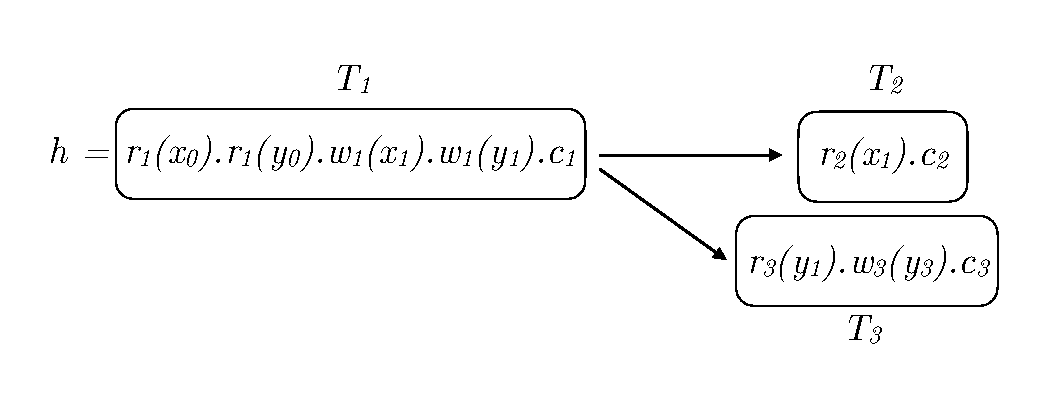
\includegraphics[width=0.7\textwidth]{figures/history.pdf}
  \vspace{-1cm}
  \caption{Example of history represented as a graph. Arrows represent the causal dependencies between operations. Adapted from \em{Ardekani et al.~\citep{ardekani-nsmi}}}
  \label{fig:history}
\end{figure}

Figure~\ref{fig:history} above shows an example, with $\tx_1 \hb_h \tx_3$ and $\tx_1 \hb_h \tx_2$. We say that two transactions $\tx_i$ and $\tx_j$ are \textbf{\em concurrent} in $h$ (denoted by $\tx_i \parallel \tx_j$) if neither $\tx_i \hb_h \tx_j$ nor $\tx_j \hb_h \tx_j$. In the figure above, $\tx_2$ and $\tx_3$ are concurrent.

\section{Consistency Models}

In this section, we define what a consistency model is, distinguishing between \emph{strong} and \emph{weak} models. We give an overview of several models, and compare them in terms of their undesirable effects.

We define a consistency model as a set of histories $\Cons$, such that $\Cons \subseteq \Hist$. Intuitively, a consistency model \emph{constrains} the set of possible histories by specifying how operations interleave in any given history. We say that a given history $h$ \emph{satisfies} a consistency model $\Cons$ if $h \in \Cons$, and that $h$ \emph{violates} $\Cons$.

In the context of databases, the definition of a consistency model maps to the concept of an \emph{isolation level} (I in AC\underline{I}D), which specifies the degree to which concurrent transactions in a database are aware of each other~\citep{adya_thesis}. We use the term consistency throughout this thesis, in accordance with Adya~\citep{adya_thesis}.

Traditionally, the different consistency models have been defined in terms of \emph{anomalies}~\citep{sql-critique}, that map to a set of undesirable histories that are observable by the system. Intuitively, we can distinguish between \emph{strong} and \emph{weak} consistency models depending on the number of anomalies they disallow, with stronger models restricting the set of possible histories more than weak ones. In the sections that follow, we give a brief overview of the traditional anomalies following the definitions advanced by Berenson et al.~\citep{sql-critique}, as well as different consistency models that preclude them. Figure~\ref{fig:anomalies} shows a quick summary of the models and anomalies we cover.

\begin{figure}[h]
\begin{center}
\begin{tabularx}{\linewidth}{ >{\centering}p{8cm} | *{5}{>{\centering}X}}
    \multirow{2}{*}{\em Anomalies} & \multicolumn{5}{c}{Consistency Models} \tabularnewline \cline{2-6}
    & SER & SI & PSI & NMSI & RC \tabularnewline \hline
    Dirty Write & x & x & x & x & x \tabularnewline
    Dirty Read & x & x & x & x & x \tabularnewline
    \hline % Distinguish between ACID or not
    Non-Repeatable Read & x & x & x & x & \checkmark \tabularnewline
    Lost Update & x & x & x & x & \checkmark \tabularnewline
    \hline % Distinguish between weak and strong
    Write Skew & x & \checkmark & \checkmark & \checkmark & \checkmark \tabularnewline
    Long Fork & x & x & \checkmark & \checkmark & \checkmark \tabularnewline
    Non-Monotonic Snapshot & x & x & \checkmark & \checkmark & \checkmark \tabularnewline
\end{tabularx}
\end{center}
\caption{Anomaly Comparison of Consistency Models \emph{(x}:disallowed, \checkmark:allowed\emph{)}. Adapted from \em{Ardekani et al.~\citep{ardekani-nsmi}}}
\label{fig:anomalies}
\end{figure}

\begin{definition}[Dirty Write]
A \emph{Dirty Write} occurs in a history $h$ when a transaction $\tx_i$ modifies an object $x$ that was previously modified by another pending transaction $\tx_j$. If any of the two transactions commit or abort, it is not clear what value the object $x$ should have. A Dirty Write can be represented by a history such as $w_1(x_1).w_2(x_2).(c_1 \vee a_1).(c_2 \vee a_2)$, where the termination order of the transactions can be arbitrary. The anomaly occurs even if any of the transactions aborts.
\end{definition}

\begin{definition}[Dirty Read]
A \emph{Dirty Read} occurs in a history $h$ when a transaction $\tx_i$ reads an object $x$ modified by a pending transaction $\tx_j$. If $\tx_j$ ultimately aborts in $h$, the value observed by a $\tx_i$ was never supposed to occur in $h$. This is represented by a history such as $r_1(x_0)\ldots w_1(x_1)\ldots r_2(x_1)\ldots c_2\ldots a_1$.
\end{definition}

Both of these anomalies can be prevented by making a transaction's changes visible only after it commits. For example, updates can be buffered locally in the context of a transaction. All the consistency models we describe in the sections that follow preclude dirty writes and reads. Transactions executing under such models offer \emph{atomicity} (A in \underline{A}CID).

\begin{definition}[Non-Repeatable Read]
A non-repeatable read---also called a \emph{fuzzy read}--occurs whenever a transaction $\tx_i$ observes different values for an object $x$ on subsequent read operations when interleaved by a commit by another transaction, $\tx_j$. This can be seen in $r_1(x_0)\ldots r_2(x_0).w_2(x_2).c_2 \ldots r_1(x_2)$. Here, $\tx_1$ observers two different values of $x$: the initial version $x_0$ and the version $x_2$ written by $\tx_2$.
\end{definition}

The non-repeatable read anomaly can also be prevented in an easy way: a transaction can keep a cache of already read values. Subsequent read operations can return values from this read cache.

\begin{definition}[Lost Update]
A \emph{Lost Update} occurs in a history $h$ when two concurrent transactions update the same object $x$ and successfully commit. In this case, the update written by whichever transaction commits first is ``lost'' after the second transaction commits. This can be seen in a history such as $r_1(x_0)\ldots r_2(x_0).w_2(x_2) \ldots w_1(x_1).c_1\ldots c_2$. After $\tx_2$ commits, version $x_1$ will no longer be visible to subsequent transactions.
\end{definition}

For the purposes of this thesis, and following the definition proposed in Ardekani et al.~\citep{ardekani_thesis}, we say that a consistency model is \emph{strong} if it prevents concurrent transactions to modify the same object. That is to say, a strong consistency model preclude dirty writes and reads, along with lost update anomaly. A model that allows concurrent transactions to modify the same object is \emph{weak}.

We now review several well-known strong consistency models, along with a weak model that will serve as a baseline comparison in the following chapters.

\subsection{Serialisability}

Serialisability restricts the set of possible histories to those equivalent to some \emph{serial} execution. That is to say, under a traditional system offering Serialisability, the happens-before relation we introduced in~\ref{sect:histories} is a \emph{strict total order} \todo{does it need to be strict?}. A history such as the one in Figure~\ref{fig:history} is serialisable, because we can order $\tx_2$ to occur before $\tx_3$ (or vice versa); while the one shown in Figure~\ref{fig:non_ser_history} is not.

\subsection{Snapshot Isolation}
\subsection{Parallel Snapshot Isolation}
\subsection{Non-Monotonic Snapshot Isolation}
\subsection{Read Committed}

\section{Catalog of Protocols}
\subsection{Walter}
\subsection{Jessy}
% \subsection{GMU} Tentative, since we don't talk about US in previous section

   \cleardoublepage
\chapter{PSI/NMSI}

\todo{
We explain what PSI is, how it differs from classical SI, and how it avoids some of the anomalies explained during the preliminaries. Explain the protocol in terms of abstract executions. As Alexey for reference showing that PSI is equivalent to NMSI.

PSI = SI within a site, (isolation) + causal consistency across sites (consistency) => ref Lamport.

Traditional SI = Sequential consistency?.

Mention~\citep{psi-intro}, difference: transactions are not fixed at start time, but at read time (like NMSI).

From same paper:

Snapshot isolation is inadequate for a system replicated at many sites, due to two issues. First, to define snapshots, snapshot iso- lation imposes a total ordering of the commit time of all transac- tions, even those that do not conflict. Establishing such an ordering when transactions execute at different sites is inefficient. Second, the writes of a committed transaction must be immediately visible to later transactions. Therefore a transaction can commit only after its writes have been propagated to all remote replicas, thereby pre- cluding asynchronous propagation of its updates.
}

   \cleardoublepage
\chapter{The Protocol}
\label{protocol_chapter}

\newcommand{\Wconflict}{\text{\sc Conflict}\xspace}

\newcommand{\Obj}{{\sf Obj}}
\newcommand{\partitions}{\ensuremath{\mathsf{partitions}}}
\newcommand{\TxVars}{\ensuremath{\mathsf{TxVars}}}
\newcommand{\Tvar}{\ensuremath{\mathsf{T}}}
\newcommand{\Svar}{\ensuremath{\mathsf{S}}}
\newcommand{\Clients}{\ensuremath{\mathsf{Clients}}}
\newcommand{\Partitions}{\ensuremath{\mathsf{Partitions}}}
\newcommand{\VCSet}{\ensuremath{\mathsf{VerVector}}}
\newcommand{\VCType}{\ensuremath{\mathit{V}}}
\newcommand{\WSType}{\ensuremath{\mathit{WS}}}

\newcommand{\MsgLabel}{\ensuremath{\mathsf{MessageLabels}}}
\newcommand{\Messages}{\ensuremath{\mathsf{Messages}}}

\newcommand{\localWS}{\ensuremath{\mathit{WS}}}
\newcommand{\partitionOf}{\ensuremath{\mathsf{partition}}}
\newcommand{\WS}{\ensuremath{\mathsf{WS}}}
\newcommand{\WriteSets}{\ensuremath{\mathsf{WriteSets}}}

\newcommand{\Tx}{\ensuremath{\mathsf{Tx}}}
\newcommand{\VCdep}{\ensuremath{\mathsf{Vdep}}}
\newcommand{\VCaggr}{\ensuremath{\mathsf{Vsnap}}}
\newcommand{\Vaggr}{\ensuremath{\mathsf{Vaggr}}}
\newcommand{\Value}{\ensuremath{\mathsf{Value}}}
\newcommand{\CommitTime}{\ensuremath{\mathsf{CommitTime}}}
\newcommand{\Vcomm}{\ensuremath{\mathsf{Vcomm}}}

\newcommand{\Versions}{\ensuremath{\mathsf{Versions}}}
\newcommand{\pending}{\text{\sc pending}}
\newcommand{\ready}{\text{\sc decided}}
\newcommand{\CQentries}{\ensuremath{\mathsf{CQentries}}}
\newcommand{\CLogs}{\ensuremath{\mathsf{CLogs}}}
\newcommand{\VLogs}{\ensuremath{\mathsf{Vlogs}}}
\newcommand{\PState}{\ensuremath{\mathsf{PState}}}

\newcommand{\CommitLog}{\ensuremath{\mathsf{CommitLog}}}
\newcommand{\CommitQueue}{\ensuremath{\mathsf{CommitQueue}}}
\newcommand{\VersionLog}{\ensuremath{\mathsf{VersionLog}}}
\newcommand{\LastTransactionProcessed}{\ensuremath{\mathsf{LastPrep}}}
\newcommand{\LocalTime}{\ensuremath{\mathsf{Vtotal}}}
\newcommand{\LocalEntry}{\ensuremath{\mathit{MVC}}}
\newcommand{\hasRead}{\ensuremath{\mathsf{HasRead}}}

\newcommand{\VCzero}{\ensuremath{\mathbf{0}_V}}
\newcommand{\dom}{\ensuremath{\mathsf{dom}}}

\newcommand{\Cevent}{\ensuremath{\mathsf{ConcEvents}}}
\newcommand{\actionOf}{\ensuremath{\mathsf{ActionOf}}}
\newcommand{\Act}{\ensuremath{\mathsf{Act}}}
\newcommand{\actstart}{\ensuremath{\mathsf{start}}}
\newcommand{\actwrite}{\ensuremath{\mathsf{write}}}
\newcommand{\actread}{\ensuremath{\mathsf{read}}}
\newcommand{\actreadreturn}{\ensuremath{\mathsf{read}\_\mathsf{return}}}
\newcommand{\actabort}{\ensuremath{\mathsf{abort}}}
\newcommand{\actreadrequest}{\ensuremath{\mathsf{read}\_\mathsf{request}}}
\newcommand{\actwritetolog}{\ensuremath{\mathsf{writeToVlog}}}
\newcommand{\actcommit}{\ensuremath{\mathsf{commit}}}
\newcommand{\actcommitreturn}{\ensuremath{\mathsf{commit}\_\mathsf{return}}}
\newcommand{\actprepare}{\ensuremath{\mathsf{prepare}}}
\newcommand{\actdecide}{\ensuremath{\mathsf{decide}}}
\newcommand{\actupdate}{\ensuremath{\mathsf{update}}}

\newcommand{\TxNew}{\ensuremath{\mathsf{TxNew}}}
\newcommand{\TxWrite}{\ensuremath{\mathsf{TxWrite}}}
\newcommand{\TxFirstRead}{\ensuremath{\mathsf{TxFirstRead}}}
\newcommand{\TxOtherRead}{\ensuremath{\mathsf{TxOtherRead}}}
\newcommand{\TxReadAbort}{\ensuremath{\mathsf{TxReadAbort}}}
\newcommand{\TxReadSuccessful}{\ensuremath{\mathsf{TxReadSuccess}}}
\newcommand{\TxReadRequestOld}{\ensuremath{\mathsf{TxOldReadRequest}}}
\newcommand{\TxReadRequestNew}{\ensuremath{\mathsf{TxNewReadRequest}}}
\newcommand{\TxReadRequestAbort}{\ensuremath{\mathsf{TxAbortReadRequest}}}
\newcommand{\TxReadOnlyCommit}{\ensuremath{\mathsf{TxReadOnlyCommit}}}
\newcommand{\TxStartCommit}{\ensuremath{\mathsf{TxStartCommit}}}
\newcommand{\TxEndCommit}{\ensuremath{\mathsf{TxEndCommit}}}
\newcommand{\TxWriteConflictConcurrent}{\ensuremath{\mathsf{TxWWConfConcurrent}}}
\newcommand{\TxWriteConflictCommitted}{\ensuremath{\mathsf{TxWWConfCommitted}}}
\newcommand{\TxNoWriteConflict}{\ensuremath{\mathsf{TxNoWWConf}}}
\newcommand{\TxDecideTrue}{\ensuremath{\mathsf{TxDecideTrue}}}
\newcommand{\TxDecideFalse}{\ensuremath{\mathsf{TXDecideFalse}}}
\newcommand{\TxUpdate}{\ensuremath{\mathsf{TxUpdate}}}

\newcommand{\msgreadrequest}{\ensuremath{\mathsf{READREQUEST}}}
\newcommand{\msgreadreturn}{\ensuremath{\mathsf{READRETURN}}}
\newcommand{\msgprepare}{\ensuremath{\mathsf{PREPARE}}}
\newcommand{\msgdecide}{\ensuremath{\mathsf{DECIDE}}}
\newcommand{\msgvote}{\ensuremath{\mathsf{VOTE}}}

\newcommand{\lastCompatibleVersion}{\ensuremath{\mathsf{lastCompatible}}}
\newcommand{\fixSnapshot}{\ensuremath{\mathsf{fixSnapshot}}}
\newcommand{\updateCommitVC}{\ensuremath{\mathsf{CommitVC}}}

\newcommand{\CommitVector}{\ensuremath{\mathsf{CommitVC}}}

\newcommand{\abort}{\text{\sc abort}}
\newcommand{\commit}{\text{\sc commit}}

\newcommand{\access}{\ensuremath{\mathsf{Access}}}

\newcommand{\TO}{\ensuremath{\mathsf{to}}}

\newcommand{\startEvent}{\ensuremath{\mathsf{startEvent}}}

\newcommand{\readmessages}{\ensuremath{\mathsf{readMessages}}}
\newcommand{\commitmessages}{\ensuremath{\mathsf{commitMessages}}}
\newcommand{\updatemessages}{\ensuremath{\mathsf{updateMessages}}}

\newcommand{\vlsubseteq}{\ensuremath{\sqsubseteq_{\mathsf{VL}}}}
\newcommand{\dvsubseteq}{\ensuremath{\sqsubseteq_{\mathsf{VC}}}}

\newcommand{\lastVC}{\ensuremath{\mathsf{lastVC}}}

\newcommand{\at}{\ensuremath{@}}

\newcommand{\localVaggr}{\mathit{Vaggr}}
\newcommand{\localVdep}{\mathit{Vdep}}
\newcommand{\argVCaggr}{\ensuremath{\mathit{Vsnap}}}
\newcommand{\argVCdep}{\ensuremath{\mathit{Vdep}}}
\newcommand{\argHasRead}{\mathit{HasRead}}
\newcommand{\argCommitVC}{\ensuremath{\mathit{commitVC}}}
\newcommand{\maxVC}{\ensuremath{\mathit{MaxVC}}}
\newcommand{\argMaxVC}{\ensuremath{\mathit{MaxVC}}}
\newcommand{\argVLog}{\ensuremath{\mathit{VersionLog}}}

\newcommand{\READREQUEST}{{\tt READREQUEST}}
\newcommand{\READRETURN}{{\tt READRETURN}}
\newcommand{\PREPARE}{{\tt PREPARE}}
\newcommand{\DECIDE}{{\tt DECIDE}}
\newcommand{\VOTE}{{\tt VOTE}}
\newcommand{\ABORT}{{\tt ABORT}}

\newcommand{\outcome}{\mathit{decision}}
\newcommand{\false}{\bottom}
\newcommand{\true}{\top}

\newcommand{\cqueue}{\CommitQueue}
\newcommand{\cqhead}{\CommitQueue.{\sf head}}
\newcommand{\cqupdate}{\CommitQueue.{\sf update}}
\newcommand{\cqremove}{\CommitQueue.{\sf remove}}
\newcommand{\cqput}{\CommitQueue.{\sf put}}

\newcommand{\cladd}{\CommitLog.{\sf add}}

\newcommand{\vlapply}{\VersionLog.{\sf add}}
\newcommand{\vllast}{\VersionLog.{\sf last}}
\newcommand{\last}{{\rm last}}
\newcommand{\ver}{\mathit{ver}}

\newcommand{\mrvc}{\LocalTime}

\newcommand{\lastprep}{\LastTransactionProcessed}

\newcommand{\parti}{\mathit{p_i}}
\newcommand{\partj}{\mathit{s_j}}

\newcommand{\transtype}{{\sf Tx}}
\newcommand{\keytype}{{\sf Object}}
\newcommand{\valuetype}{{\sf Value}}
\newcommand{\vctype}{{\sf VerVector}}

\newcommand{\val}{{\sf val}}

\newcommand{\tx}{\ensuremath{\mathit{T}}}

\newcommand{\commitVC}{\mathit{Vcomm}}

\newcommand{\localkey}{{\sf k}}
\newcommand{\localval}{{\sf v}}
\newcommand{\partitionof}{{\sf partition}}

\SetKwBlock{SubAlgoBlock}{}{end}
\newcommand{\SubAlgo}[2]{#1 \SubAlgoBlock{#2}}

\SetKw{Upon}{upon}
\SetKw{WhenReceived}{when received}
\SetKw{Send}{send}
\SetKw{Receive}{wait receive}
\SetKw{Until}{wait until}
\SetKw{KwFrom}{from}
\SetKw{KwTo}{to}
\SetKw{Throw}{throw}
\SetKw{Fun}{function}
\SetKw{Break}{break}
\SetKw{New}{new}

% Go over the different parts of the protocol, or at least the read request and prepare/decide.

% We should talk something about prefix order and read aborts here. Image of the executions that cause read aborts.

\todo{Protocol name?}

In this chapter, we describe how our protocol works. We first present how the system is modelled, followed by a description of the different data data structures that it encompasses. Next, we show how the protocol is implemented by going over the execution of a transaction, focusing in particular on the read and commit phases.

\section{System Model}

We consider an asynchronous, message-passing system consisting of a set of reliable processes connected by reliable channels. Fault-tolerance concerns are orthogonal to the problem we address. The processes are split into two sets; a set of \emph{servers} $\mathcal{S} = \{s_1, \dots, s_N\}$, and a set of \emph{clients} $\mathcal{C} = \{c_1, \dots, c_M\}$. The system manages a set of objects $\Obj$ split into $N$ partitions, each stored by a server process. We let $\partitionOf(x)$ be the index of the partition the object $x$ belongs to, so that it is managed by server $s_{\partitionOf(x)}$. Clients execute transactions by communicating with servers. Transactions can be \emph{interactive}, i.e., when a transaction starts, the client does not know which operations it will perform in advance. Clients refer to transactions by their identifier from a set $\transtype$.

\section{Server data structures}

The data structures maintained by the protocol at a process are summarised in Figure~\ref{fig:prot-ds-table}. Each server $s_i$ maintains a counter $\lastprep$ of the number of update transactions that initiated their commit phase at the server. When such a transaction commits at a server $s_i$, it will be assigned a \emph{sequence number} $k$ derived from this counter. All the update operations by the transaction at $s_i$ are identified by a pair $(s_i, k)$, which we call dot~\citep{carlos-causality}. We call the order of transactions imposed by their sequence numbers issued by $s_i$ the \emph{commit order} at $s_i$.

To track the happens-before relationship between transactions, we use \emph{version vectors}~\citep{version-vectors}. Such a vector consists of $n$ entries, each for each server, storing a non-negative integer. A version vector $V$ represents the set of dots $\{(s_i, k) \mid k \le V[i]\}$, which identify the writes by transactions whose sequence number at a server $s_i$ is no higher than $V[i]$. Version vectors are compared according to the following relation, showing when one vector covers more dots than another: $V_1 \sqsubseteq V_2 \iff \forall i.\ V_1[i] \le V_2[i]$. In addition, there exists a \emph{join} operation on vectors, taking their component-wise maximum. We we will denote this operation by $\max$ from now on. We also denote the set of all version vectors by $\VCSet$, and the vector with all entries set to $0$ by $\vec{0}$.

The protocol associates each committed transaction $\tx$ with a \emph{commit vector}---a version vector $V$ representing the dots that cover all the writes by $\tx$ as well as the writes of transactions preceding $\tx$ under happens-before. In particular, the entry $V[i]$ for a server $s_i$ where $\tx$ wrote an object stores the sequence number of $\tx$ issued by $s_i$. A server $s_i$ maintains a list of update transactions that committed at the server in a $\CommitLog$, storing triples $\langle T,V_c,V_a\rangle$. Here, $\tx$ is the identifier of a committed transaction, and $V_c$ is its commit vector. The $\CommitLog$ at $s_i$ is totally ordered according to the value $V_c[i]$, which follows the commit order at $s_i$. The last component of the triple, $V_a$, represents the join of the commit vectors of all the transactions up to $\tx$ in $\CommitLog$. This \emph{aggregate} vector is stored for efficiency---the server also caches the aggregate vector of the last committed transaction in a variable $\LocalTime$. Initially, the $\CommitLog$ contains a single dummy entry $\langle \_, \vec{0}, \vec{0} \rangle$.

A server $s_i$ maintains multiple versions of the objects it manages, stored in a mapping $\VersionLog$, which we call the \emph{database}. This log maps an object to a a list of \emph{versions}, pairs of a value and the commit vector of the transaction that wrote this value. The $\VersionLog$ is ordered by the $i$-th component of the commit vector of each version, which follows the commit order of transactions at $s_i$. We denote by $\VersionLog[x].\last$ the most recent entry in the list for the object $x$.

Finally, a server $s_i$ maintains an ordered queue $\CommitQueue$ of transactions trying to commit updates at the server. The queue has entries of two types. An entry $\langle \pending, T, \localWS \rangle$ means that $\tx$ is successfully prepared to commit at $s_i$, but the final decision on it is not yet known; $\localWS$ is the \emph{write-set} of the transaction, containing object-value pairs. An entry $\langle \ready, T, \localWS, V \rangle$ in the queue means that $\tx$ has been decided to commit with a commit vector $V$, but its writes have not yet been added to the $\VersionLog$. The order of transactions in $\CommitQueue$ follows the commit order at the server.

\section{Transaction Execution}

\todo{Maybe it's better to split the pseudocode and inline it with the text?}

\todo{Maybe we should go over how snapshots are built, and explain how they can abort, before going over a sample execution.}

\subsection{Reading Objects and Building Consistent Snapshots}

A client executing a transaction $\tx$ maintains a transaction \emph{context} including several pieces of data, summarised in Figure~\ref{fig:prot-ds-table} and explained below. This context is initialised by the client when it starts a transaction (line~\ref{alg:start_tx_start}).

Since our protocol uses optimistic concurrency control, the execution of $\tx$ is speculative: clients read objects from servers and buffer writes locally. At the end of the execution, the decision whether to commit or abort a transaction is taken based on the existence of conflicts with concurrently executing transactions. When a transaction $\tx$ writes a value $v$ to an object $x$ (line~\ref{alg:write_start}), the client buffers this write in $\tx$'s \emph{write-set}, $\tx.\WS$, while discarding any previously written value of $x$.

When the transaction $\tx$ issues a read operation on an object $x$ (line~\ref{alg:read_start}), the client will first check $\tx.\WS$ (line~\ref{alg:read_ws_check}): if $\tx$ has already written to $x$, the value stored in the write-set is returned. Otherwise, and assuming that $j = \partitionOf(x)$, the client sends a $\READREQUEST$ message to the server $s_j$ to fetch the value of the object (line~\ref{alg:read_send}).

When the transaction $\tx$ reads an object from a partition $j$ for the first time, the server $s_j$ fixes a \emph{snapshot} of versions from which it will serve all future reads by $\tx$. This snapshot is defined by an integer $k$: it will include the versions written by all the transactions that committed at the server with a sequence number up to $k$. The client keeps this information in the transaction context, by storing $k$ in the $j$-th entry of a \emph{snapshot vector} $\tx.\VCaggr$, and by marking the current partition as read in $\tx.\hasRead$, a Boolean mapping its $j$-th entry to $\top$ if $\tx$ read an object from $j$, and $\bot$ otherwise. If $\tx.\hasRead[j]=\top$, then the vector $\tx.\VCaggr$ is equal to the join of the commit vectors of all transactions that at partition $j$ have a sequence number no higher than $\VCaggr[j]$, and vice versa.

\todo{This is the first time that causal dependency is mentioned.} Thus, the entries of the snapshot vector for partitions that $\tx$ has not yet read from delimit all the possible causal dependencies $\tx$ may develop at these partitions if it keeps reading objects from the snapshots it has already fixed.

Both $\tx.\VCaggr$ and $\tx.\hasRead$ are supplied by the client when issuing a read operation on object $x$, by using them as parameters to the $\READREQUEST$ message sent to the server $s_j$. When the server receives this message (line~\ref{alg:read_req_start}), it first checks, using the $\hasRead$ mapping, if the transaction has read from it before (line~\ref{alg:read_req_read_check}). In this case, the snapshot is determined by $\VCaggr[j]$, and the server returns the latest version $\mathit{ver}$ of the object $x$ written by a transaction in the snapshot, i.e., with a sequence number no higher than $\VCaggr[j]$ (line~\ref{alg:chose-version}). This version is determined by examining the $j$-th entry of the commit vectors in $\VersionLog$. The server then replies to the client with a $\READRETURN$ message containing the value of the chosen version and its associated version vector, as well as the unmodified snapshot vector provided by the client: since the server used a previously fixed snapshot, no updates to the vector are required.

% \begin{figure}[t]
% 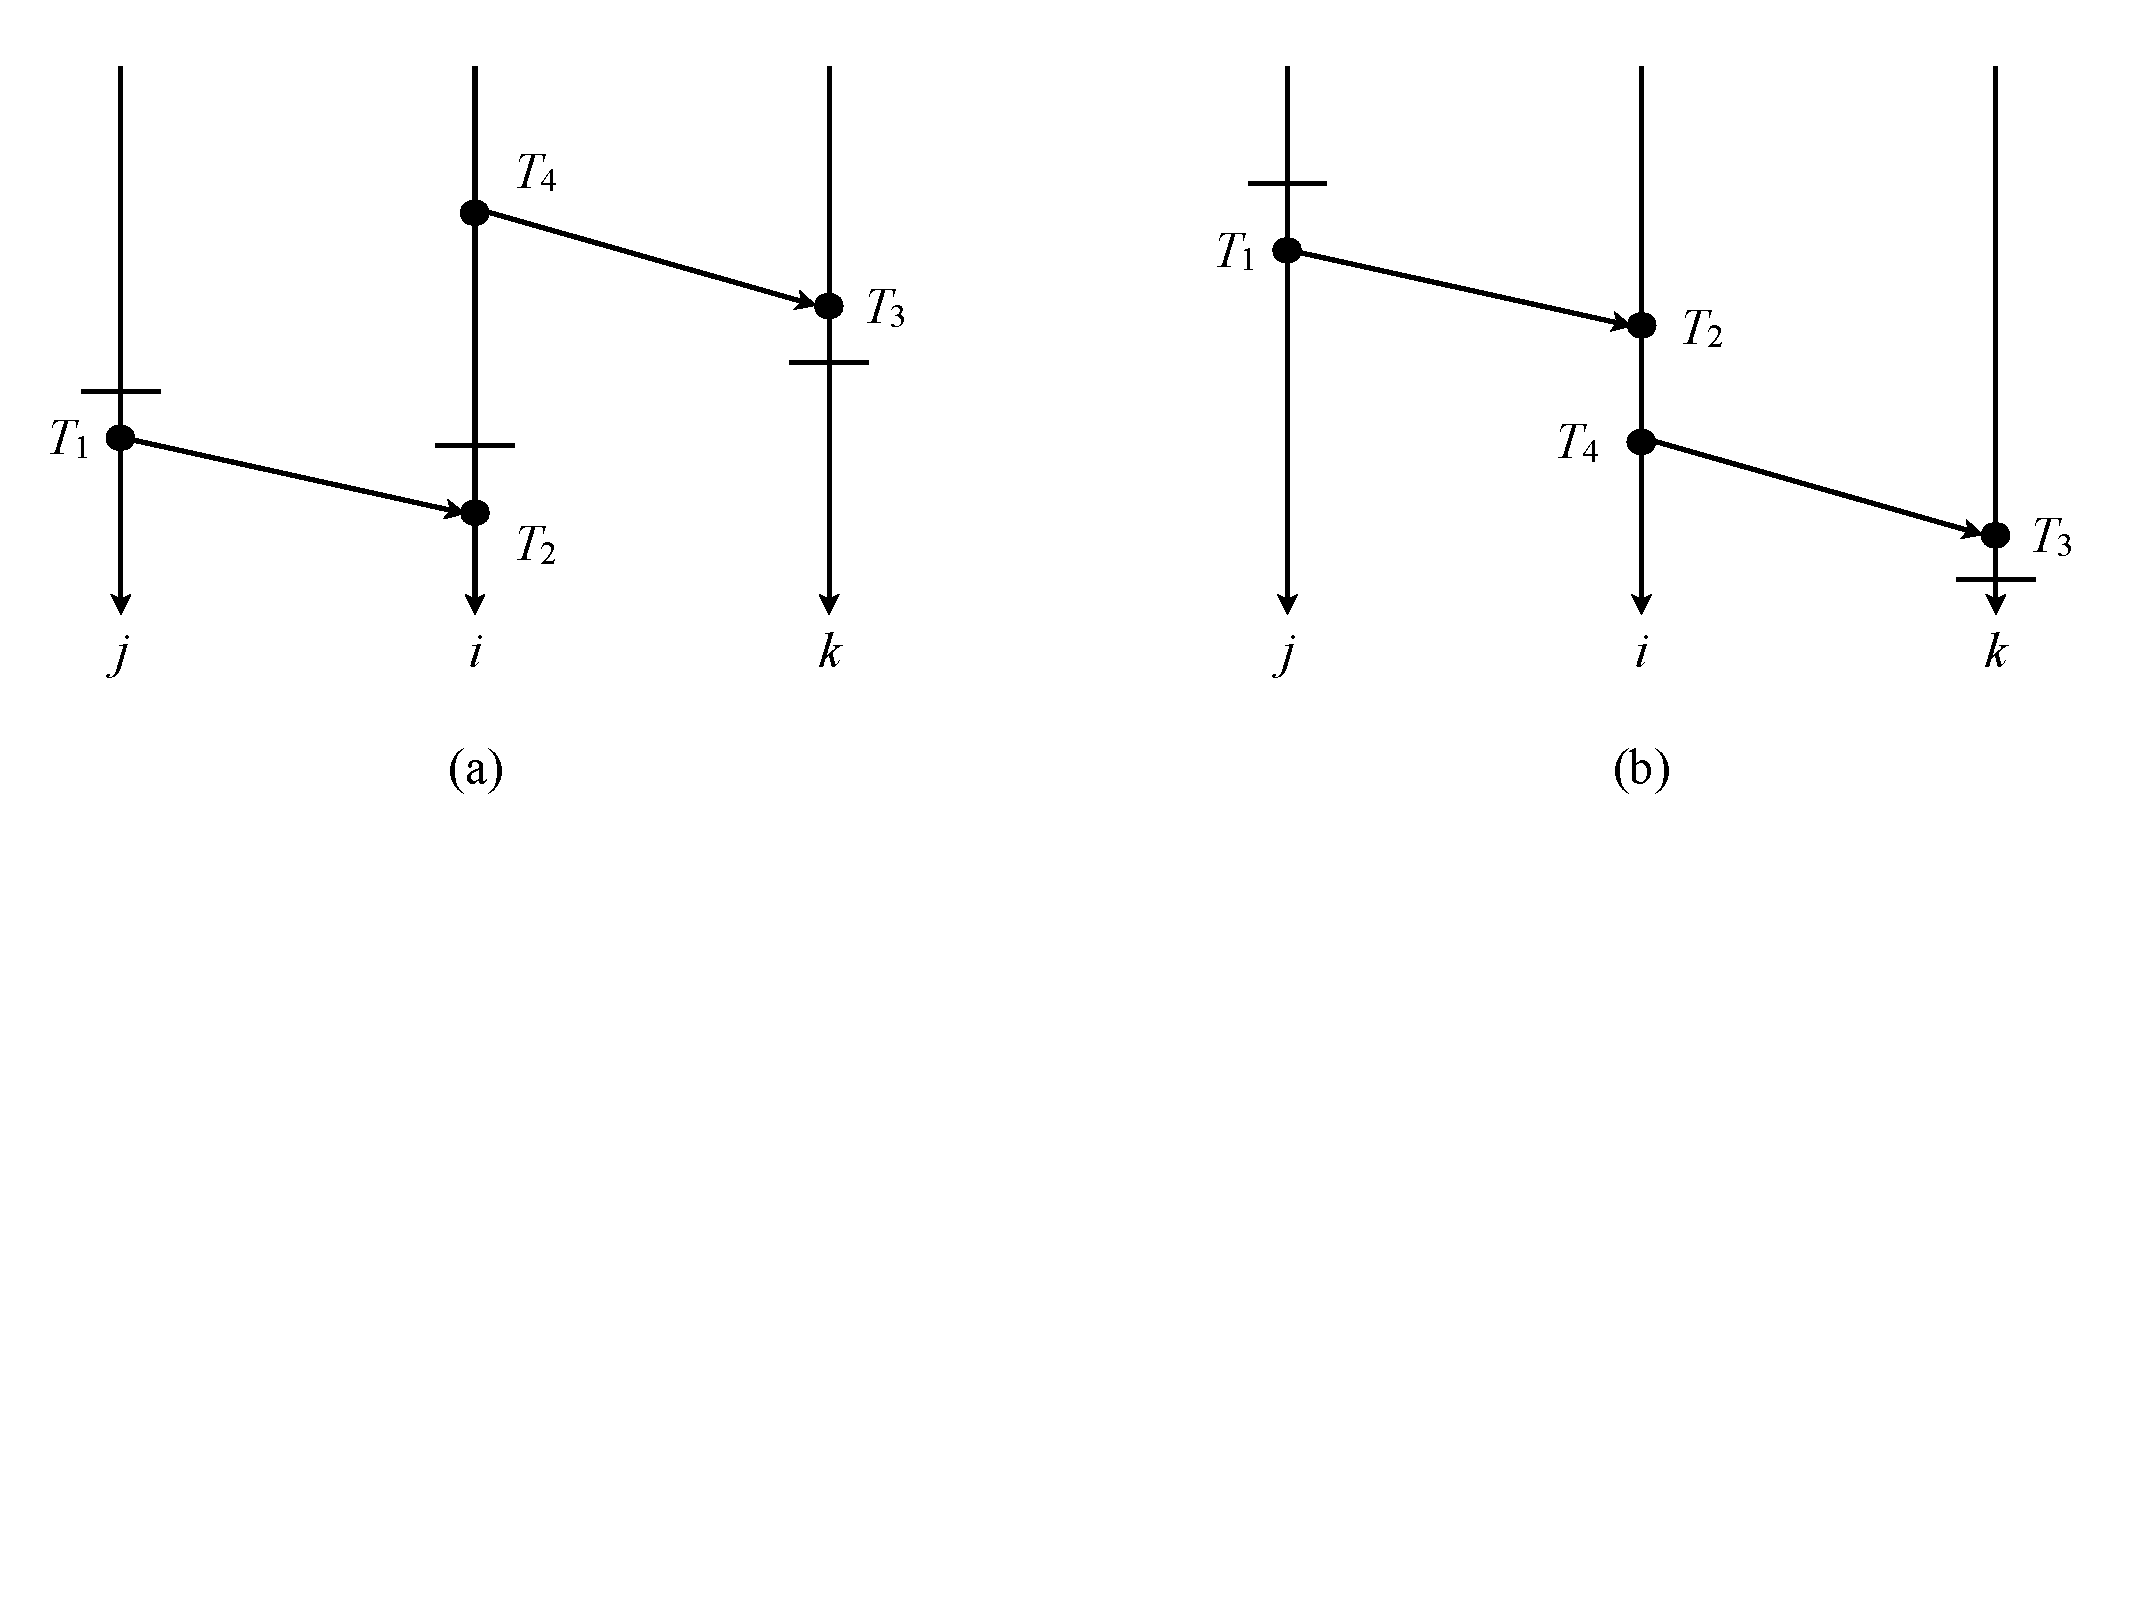
\includegraphics[width=\textwidth]{figures/ch4_snapshot.pdf}
% \vspace{-6.5cm}
% \caption{Illustrations of the snapshot computation. Vertical lines depict the
%   commit order at the corresponding partitions (top to bottom) and horizontal
%   lines the cut-offs of various snapshots. Arrows between partitions depict
%   causal dependencies.}
% \label{fig:snapshot}
% \end{figure}

% \begin{figure}[t]
% 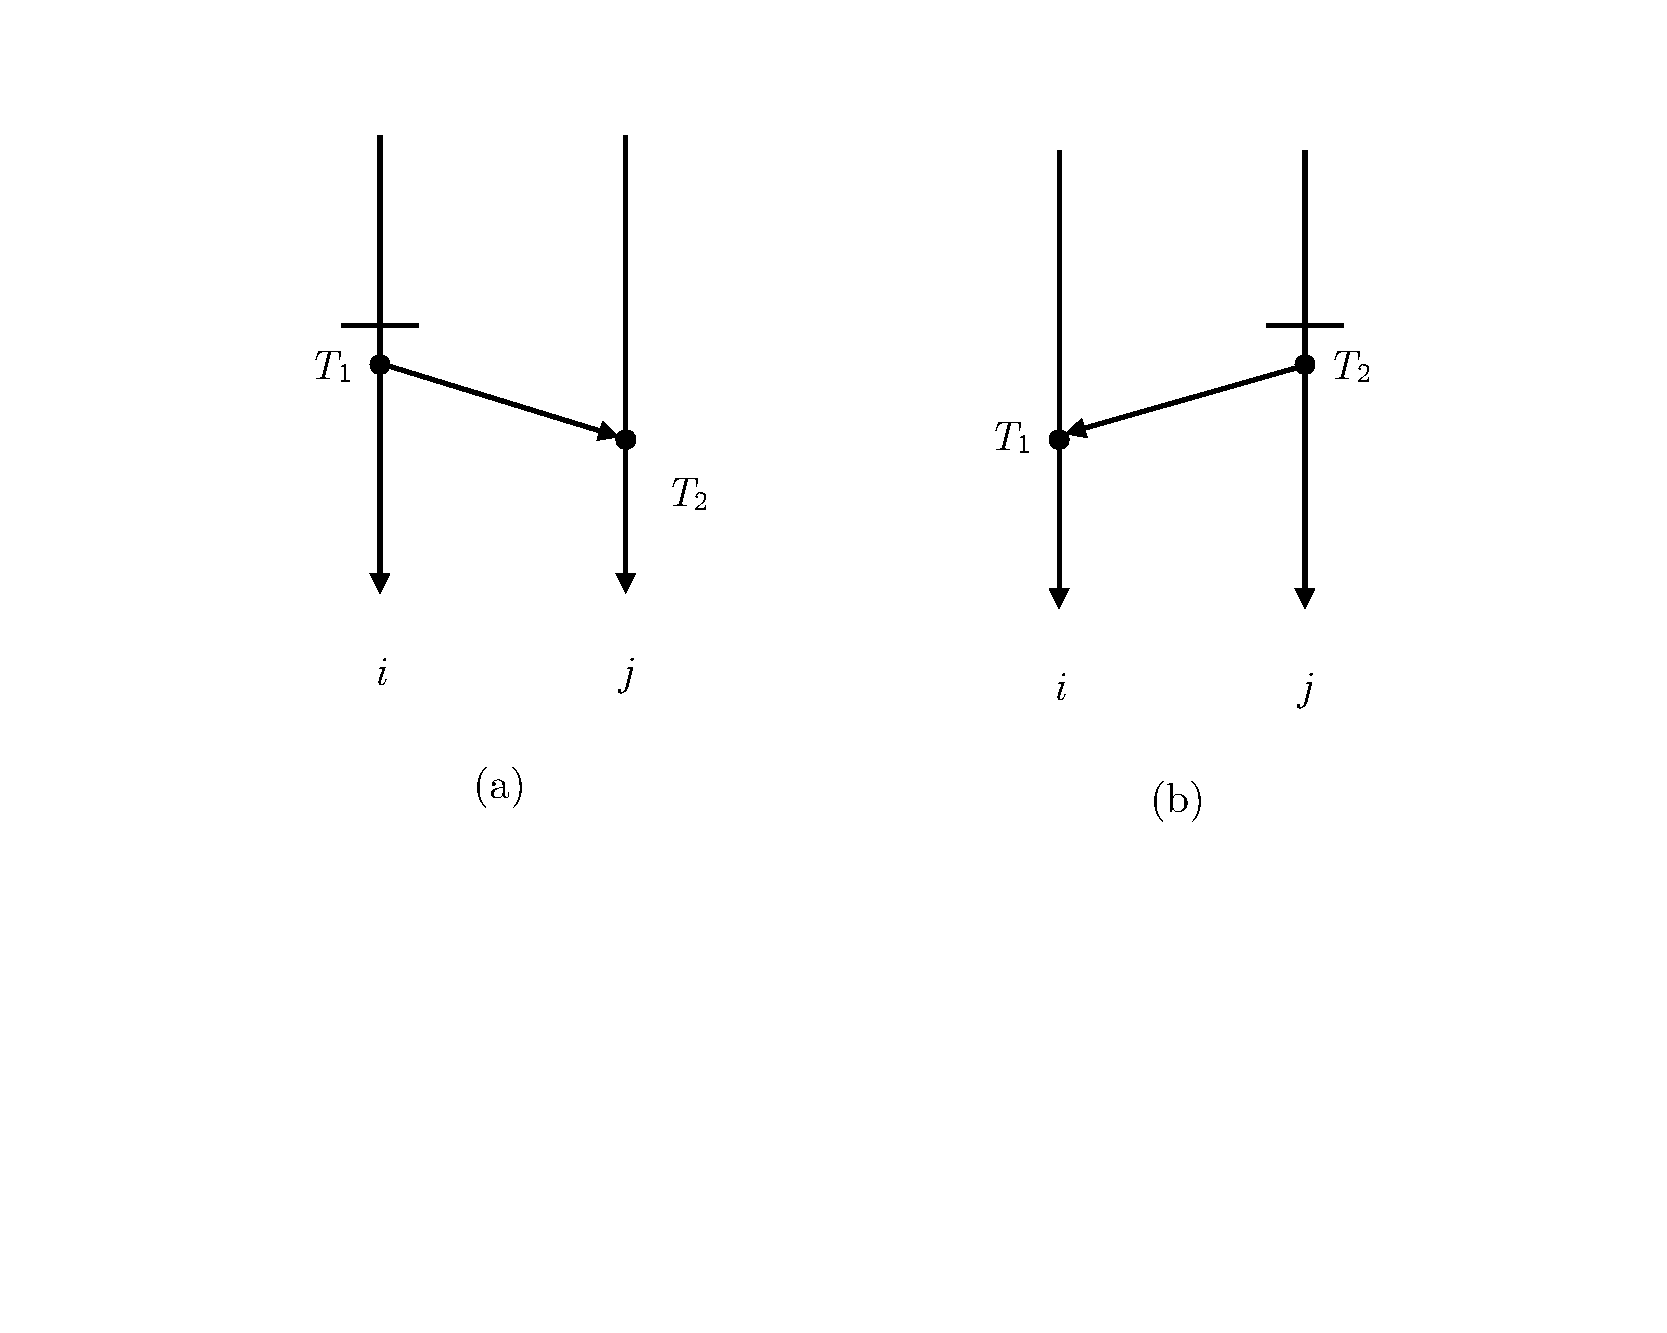
\includegraphics[width=\textwidth]{figures/ch4_snapshot_fork.pdf}
% \vspace{-5.5cm}
% \caption{Illustrations of the snapshot computation. Vertical lines depict the
%   commit order at the corresponding partitions (top to bottom) and horizontal
%   lines the cut-offs of various snapshots. Arrows between partitions depict
%   causal dependencies.}
% \label{fig:fig:snapshot_fork}
% \end{figure}

We now consider the case when the client is reading from the server $s_j$ for the first time (line~\ref{alg:read_req_read_check_else}), in which case, we have to fix the snapshot for the transaction $\tx$ at this server. Choosing a suitable snapshot is complicated by the fact that we allow transactions to be interactive---that is, we do not know in advance which objects will read in the future. We hence fix the snapshot in such a way that \emph{any} later read from this snapshot will be causally \todo{cc} compatible with any reads (past or future) from the snapshots that $\tx$ has already read, as specified by $\hasRead$ and $\VCaggr$. To ensure this, the snapshot we select has to satisfy two requirements.

\todo{snip: insert two requirements. Example of simple read abort?}

Once the server fixes a new snapshot, it selects the most recent version of the object $x$, defined by $e.\Vaggr[j]$ (line~\ref{alg:chose-version}), to return to the client. The server replies with a $\READRETURN$ message, carrying a triple of the value of the object, its associated version vector, and the aggregate vector for $e.\Vaggr$, summarising the causal \todo{cc} dependencies of all the transactions in the snapshot. When the client receives the message (line~\ref{alg:read_msg_decomp}), it first sets the $j$-th entry of $\tx.\hasRead$ to $\top$, to indicate that $\tx$ has read an object at partition $j$, and joins the returned aggregate vector to $\tx.\VCaggr$. The client also joins the commit vector associated with the version read to a \emph{dependency vector} $\tx.\VCdep$, which represents all causal \todo{cc} dependencies developed by $\tx$ during its execution. This ensures that, upon reading a version of object $x$, $\tx$ will causally depend \todo{cc} on the transaction $\tx'$ that wrote that version of $x$, along with the causal dependencies of $\tx'$.

\todo{Verify that we mentioned read aborts in this section}

\subsection{Transaction Termination}

A client executing a transaction $\tx$ tries to commit it by calling a {\tt commit} function (line~\ref{alg:commit_start}). Read-only transactions are committed without any additional checks, since they already read a causally consistent snapshot (line~\ref{alg:commit_readonly_start}) \todo{define causally consistent snapshot}. To commit an update transaction $\tx$, we use a variant of the classical \emph{two-phase commit protocol (2PC)} \todo{cite 2PC?} among the processes that store the objects written by the transaction; the client executing $\tx$ servers as the 2PC coordinator.

In more detail, to commit a transaction $\tx$, the client first sends a $\PREPARE$ message to all servers storing the objects written by the transaction (line~\ref{alg:commit_send_loop}). The message contains $\tx$'s write-set and its dependency vector $\tx.\VCdep$. When a server $s_i$ receives this message (line~\ref{alg:prepare_start}), it \emph{validates} the transaction, deciding whether it can commit or abort due to conflicting concurrent transactions. The server then replies to the client with a \emph{vote} representing its decision. Based on the votes, the client determines the final decision on the transaction---the transaction commits if all votes are positive---and distributes the decision to the relevant servers.

We now describe how a server $s_i$ computes its vote on a transaction (line~\ref{alg:conflict_check}). The vote for a transaction $\tx$ ensures the following property, used to validate the \Wconflict axiom of PSI: \todo{Reference back to the model in previous chapter}

\begin{itemize}
    \item \emph{For any pair of distinct transactions $\tx_1$ and $\tx_2$ writing to an object $x$, if $\tx_1$ precedes $\tx_2$ in the commit order, then $\tx_2$ will se the version of $x$ at least as up-to-date as the one written by $\tx_1$.}
\end{itemize}

To ensure this property, the server $s_i$ first check whether, for the objects that $\tx$ wrote to, the versions that $\tx$ read are still the most up-to-date ones in the database of $s_i$ at the time of validation. The server then checks whether $\tx$ conflicts with any transactions present in $\CommitQueue$, which have started committing at the server, but whose writes have not been applied to the database yet---the server aborts $\tx$ if any transaction $\tx'$ in $\CommitQueue$ writes to the same object as $\tx$. The writes in $\CommitQueue$ may be applied to the database before the writes of $\tx$, so checking for conflicts with them ensures that $\tx$'s reads will still be up-to-date when $\tx$'s writes are applied to the database.

If the validation for transaction $\tx$ fails, the server sends a $\VOTE$ message with the vote \abort, which tells the client to abort the transaction. If the validation succeeds, the server generates a sequence number for the transaction by incrementing $\lastprep$ and sends to the client a $\VOTE$ message with this sequence number and a vote \commit. The server also adds an entry $\langle \pending, \tx, \tx.\WS \rangle$ to the $\CommitQueue$, to record the fact that it is trying to commit $\tx$ at the server (lines~\ref{alg:lastprep_incr}--\ref{alg:prepare_end}).

The client waits until it receives $\VOTE$ messages from all involved servers (line~\ref{alg:commit_recv_vote}). If all the servers voted \commit, the client constructs the final commit vector for $\tx$ by changing its dependency vector $\tx.\VCdep$, so that it covers not only $\tx$'s causal dependencies \todo{ref again}, but also all its writes. These writes are identified by the sequence numbers provided by the servers as part of their $\VOTE$ messages. Thus, the commit vector is defined by setting the entries in $\tx.\VCdep$ for partitions written by $\tx$ to these sequence numbers (line~\ref{alg:commit_assign_seqn}). The client then sends a $\DECIDE$ message to all the involved servers with the final decision on $\tx$ along with its commit vector (line~\ref{alg:commit_send_decide}).

Upon receiving the decision on a transaction $\tx$ (line~\ref{alg:decide_start}), a server updates the entry associated with $\tx$ in $\CommitQueue$, to change its status to $\ready$ and record its commit vector. If the transaction is aborted, the server removes $\tx$ from the queue.

Committed transactions are applied to the database in their order in $\CommitQueue$, i.e., the commit order. When a $\ready$ transaction $\tx$ gets to the head of the queue (line~\ref{alg:queue_start}), the server dequeues it and adds its writes to $\VersionLog$, tagged with its commit vector. The server then joins $\tx$'s commit vector to $\LocalTime$, and adds the transaction to $\CommitLog$, along with $\LocalTime$ as its aggregate vector.

\section{Algorithm pseudocode}

\begin{figure}[h]
\noindent\adjustbox{max width=\paperwidth}{\footnotesize
\begin{tabularx}{\linewidth}{|c|p{5cm}|X|}
  \hline
  \multicolumn{3}{|c|}{\textbf{Variables at a server $s_i$}}\\
  \hline
  $\lastprep$ & {\sf Integer} & The number of update transactions that tried to
  commit at the server.
\\
  \hline
  $\CommitLog$
  & ${\sf Sequence}[\langle\transtype\ {\sf T},$ $\vctype\ \Vcomm, \vctype\ \Vaggr \rangle]$
  & Log of update transactions $T$ committed at the server, ordered by
  $V_c[i]$. Here $V_c$ is the commit vector of $T$ and $V_a$ is the aggregate
  vector of $T$: the join of the commit vectors of all transactions up to $T$ in
  $\CommitLog$.
\\
  \hline
  $\LocalTime$ & $\vctype$ & The join of the commit vectors of all
  transactions in $\CommitLog$.
\\
  \hline
  $\VersionLog$ & ${\sf Map}[\keytype,$ ${\sf
    Set}[\langle \valuetype\ \val, \vctype\ \Vcomm\rangle]]$ & Database:
  a mapping from objects to lists of pairs of a value and the
  commit vector of the transaction that wrote it. The lists are ordered
  by the $i$-th component of the commit vectors.
\\
\hline
  $\CommitQueue$ & ${\sf Sequence}[\langle \transtype, \pending, {\sf WriteSet} \rangle \cup
  \langle \transtype, \ready, {\sf WriteSet}, \vctype\rangle]$ &
  Queue containing information about update transactions trying to commit
  at the server.
\\
  \hline
  \multicolumn{3}{|c|}{\textbf{Context for a transaction $T$ at a client $c_i$}} \\
  \hline
  $T.\WS$ & ${\sf WriteSet}$ & Write-set of $T$.
\\
  \hline
  $T.\hasRead$ & ${\sf Vector}[{\sf Bool}]$ & Mapping showing whether $T$  has
  read a given partition.
\\
  \hline
  $T.\VCaggr$ & $\vctype$ & Snapshot vector: determines snapshots fixed at
  partitions $T$ has read from and possible causal dependencies at all other
  partitions.
  \\
  \hline
  $T.\VCdep$ & $\vctype$ & Dependency vector, representing all causal
  dependencies developed by $T$ during its execution.
\\
  \hline
\end{tabularx}
}
\caption{List of variables used in the protocol, where
  ${\sf WriteSet} = {\sf Set}[\langle \keytype, \valuetype \rangle]$. The orders
  of entries in $\CommitLog$, $\VersionLog$ and $\CommitQueue$ are consistent
  with the commit order of transactions the entries are associated with. We
  select the components of various tuples using the names given in the figure.}
\label{fig:prot-ds-table}
\end{figure}


\clearpage

\noindent{\bf Protocol at client $c_i$ or server $s_i$:}\\

\begin{algorithm*}[H]
%  \setstretch{1.20}
  \setcounter{AlgoLine}{0}

  %  Start
  \SubAlgo{\Fun ${\tt start}()$\label{alg:start_tx_start}}{
    \Return{$\KwSty{new}\ \transtype(\WS= \emptyset, \hasRead =
      \vec{\bot}, \VCaggr = \vec{0}, \VCdep =
      \vec{0})$};\label{alg:start_tx_end}}

    \smallskip

  % Write
  \SubAlgo{\Fun ${\tt write}(T, x, v)$\label{alg:write_start}}{
    $\tx.\WS \leftarrow \left(\tx.\WS\ \backslash\ \{\langle x, \_ \rangle\}\right) \cup \{\langle x,v\rangle\}$\;\label{alg:write_end}
  }

    \smallskip

  % Read
  \SubAlgo{\Fun ${\tt read}(T, x)$\label{alg:read_start}}{
    \If{$\langle x, v \rangle \in \tx.\WS$\label{alg:read_ws_check}}{
      \Return{$v$}\;
    }

    \smallskip

    $j \leftarrow \partitionof(x)$\;
    \Send{$\READREQUEST(x, T.\VCaggr, T.\hasRead)$} \KwTo $s_j$\;\label{alg:read_send}
    \Receive{$\READRETURN(m)$} \KwFrom $s_j$\;\label{alg:read_recv}
    \uIf{$m = \abort$} {
      \Throw{$\abort$}\;\label{alg:read_abort}
    }
    \ElseIf{$m = \langle v,\localVdep,\localVaggr \rangle$\label{alg:read_msg_decomp}}{
      $\tx.\hasRead[j] \leftarrow \true$\;
      $\tx.\VCdep \leftarrow \max(\tx.\VCdep,\localVdep)$\;\label{alg:read_upd_vcdep}
      $\tx.\VCaggr \leftarrow \max(\tx.\VCaggr,\localVaggr)$\;\label{alg:read_upd_vcaggr}
      \Return{$v$}\;\label{alg:read_end}
    }
  }

    \smallskip

  % ReadRequest
  \SubAlgo{\WhenReceived $\READREQUEST(x, \argVCaggr, \argHasRead)$ \KwFrom $c_j$\label{alg:read_req_start}}{
    \uIf{$\argHasRead[i]$\label{alg:read_req_read_check}} {
      $V \leftarrow \argVCaggr$\;\label{alg:read_req_read_maxvc}
    }
    \Else{\label{alg:read_req_read_check_else}
      \Until{$\mrvc[i] \ge \argVCaggr[i]$}\;\label{alg:read_req_wait}
      $r \leftarrow \max\{r \in \CommitLog \mid \forall j.\, \argHasRead[j] {\implies} \left(r.\Vaggr[j] \le \argVCaggr[j]\right)\}$\;\label{alg:max_vc_search}
      \If{$r.\Vaggr[i] < \argVCaggr[i]$\label{alg:read_req_abort_check}}{
        \Send{$\READRETURN(\abort)$} \KwTo $c_j$\;\label{alg:read_req_abort}
        \Return\;
      }
      $V \leftarrow r.\Vaggr$\;\label{alg:read_req_unread_maxvc}
    }
    $\ver = \max\{\ver \in \VersionLog \mid ver.\Vcomm[i] \le V[i]\}$\; \label{alg:chose-version}
    \Send{$\READRETURN(\ver.\val, \ver.\Vcomm,V)$} \KwTo $c_j$\;\label{alg:read_req_end}
  }
\end{algorithm*}

\clearpage

\begin{algorithm*}[H]
%  \setstretch{1.20}

  % Commit
  \SubAlgo{\Fun ${\tt commit}(T)$\label{alg:commit_start}}{
    \If{$\tx.\WS = \emptyset$\label{alg:commit_readonly_start}}{
      \Return{$\commit$}\;\label{alg:commit_readonly_end}
    }

    \ForAll{$\partj \in \partitions(\tx.\WS)$\label{alg:commit_send_loop}}{
      \Send{$\PREPARE(T, T.\WS, \VCdep)$} \KwTo $\partj$\;\label{alg:commit_send_prepare}
    }

    $\commitVC \leftarrow \tx.\VCdep$\; \label{alg:commit_commitvc_firstassignment}
    $\outcome \leftarrow \commit$\;

    \ForAll{$\partj \in \partitions(\tx.\WS)$\label{alg:commit_send_votes}}{
      \Receive{$\VOTE(m)$} \KwFrom $\partj$\;\label{alg:commit_recv_vote}
      \uIf{$m = \langle T, \abort \rangle$\label{alg:commit_vote_check}}{
        $\outcome \leftarrow \abort$\;
        \Break\;
      }
      \ElseIf{$m = \langle T, \commit, k \rangle$\label{alg:commit_vote_check_else}}{
        $\commitVC[j] \leftarrow k$\;\label{alg:commit_assign_seqn}
      }
    }

    \ForAll{$\partj \in \partitions(\tx.\WS)$}{
      \Send{$\DECIDE(\tx, \commitVC,\outcome)$} \KwTo $\partj$\;\label{alg:commit_send_decide}
    }

    \Return{$\outcome$}\;\label{alg:commit_end}
  }

    \smallskip

  % Prepare
  \SubAlgo{\WhenReceived $\PREPARE(\tx, \localWS, \localVdep)$ \KwFrom
    $c_j$\label{alg:prepare_start}}{
    \uIf{$(\exists T'.\
      (\langle T', \pending, \localWS' \rangle \in \cqueue \vee \langle T',
      \ready, \_, \_ \rangle \in \cqueue)
        \wedge{}$ $\localWS' \cap \localWS \ne
        \emptyset) \vee (\exists x.\, x \in \localWS \wedge
        \left(\VersionLog[x].\last.\Vcomm[i] > \localVdep[i]\right)$\label{alg:conflict_check}}{
      \Send{$\VOTE(t, \abort)$} \KwTo $c_j$\; \label{alg:send_abort}
    }\Else{
    $\lastprep \leftarrow \lastprep + 1$\;\label{alg:lastprep_incr}
    $\cqput(\tx, \pending)$\;\label{alg:queue_put}
    \Send{$\VOTE(\tx, \commit, \lastprep)$} \KwTo $c_j$\;\label{alg:prepare_end}
  }}

    \smallskip

  % Decide
  \SubAlgo{\WhenReceived $\DECIDE(\tx, \commitVC, \mathit{decision})$ \KwFrom
    $\partj$\label{alg:decide_start}}{
    \uIf{$\mathit{decision} = \commit$\label{alg:decide_if}}{
      $\cqupdate(\langle \tx, \ready, \_, \argCommitVC\rangle)$\;\label{arg:queue_update}
    }
    \Else{
      $\cqremove(\tx)$\;\label{alg:decide_end}
    }
  }

    \smallskip

  % Queue head
  \SubAlgo{\Upon $\langle T, \ready, \localWS, \commitVC\rangle =
    \cqhead()$\label{alg:queue_start}}{
    $\cqremove(T)$\;\label{alg:queue_end}
    \ForAll{$\{\langle x , v \rangle \mid \langle x , v \rangle \in \localWS \wedge \partitionof(x) = i\}$} { \label{alg:queue_loopws}
        $\vlapply(\langle x , v , \commitVC \rangle)$\;\label{alg:queue_vapply}
    }

    $\mrvc \leftarrow \max(\mrvc,\commitVC)$\;\label{alg:queue_mrvc}
    $\cladd(T, \mrvc)$\;\label{alg:queue_clog_add}
  }

\end{algorithm*}


   \cleardoublepage
\chapter{Implementation and Evaluation}
\label{eval_chapter}

\section{Implementation}

The \todo{protocol name} implementation has a client-side library~\citep{pvc-client} and a server~\citep{pvc-server}, written as a plug-in transactional protocol for AntidoteDB~\citep{antidote-db}, a key-value database. Both implementations were written in the Erlang programming language, with a total of 6K lines of code. AntidoteDB provides the application programmer rich data types such as \todo{list, mention CRDTs}, supports both in-memory and disk-based storage, and implements \todo{full/partial} replication. In our implementation, we constrain ourselves to a simple in-memory, key-value storage using Last-Write-Wins registers (LWWs) \todo{cite?}. In addition, we disable replication, focusing only on the distribution problem. During normal operation, the client-side library communicates with the server using Google's Protocol Buffers~\citep{protobuf}. To enhance network efficiency, client messages are transmitted in periodic batches to the servers.

We also implemented two alternative protocols that implement different consistency criteria: Read Committed (RC) and Serialisability (SER) \todo{cite}, so we can compare our experimental results.

\todo{Expand on this, maybe?}
To prevent unbounded state growth, we also implement a simple garbage collection mechanism for both $\CommitLog$ and $\VersionLog$ at each partition. \todo{More? Mention RC and SER implementations. Maybe pseudocode of the implementations can go in an appendix}.

\section{Evaluation}

\todo{Maybe we don't need these many subsections, and can summarise some of them in separate paragraphs}

\subsection{Experimental Setup}

\todo{Details of computers: Xeon E2186G, 6 cores, 12 threads. 3.80-4.70GHz, 32GB memory, 1GbE ethernet. For each server machine we use a client machine. Latency was added using tc. Preloaded with 1 million keys, payload of 256 bytes}

% Links (also see email)
% https://ark.intel.com/content/www/us/en/ark/products/134855/intel-xeon-e-2186g-processor-12m-cache-up-to-4-70-ghz.html

% https://www.supermicro.com/en/products/system/3U/5039/SYS-5039MC-H12TRF.cfm

\subsection{Throughput Micro-benchmark}

\subsection{Dynamic Workloads}

\subsection{Read Abort Rate Impact}

\todo{Maybe?}

   \cleardoublepage
\chapter{Conclusion}

\todo{
Talk about the limitations of our approach, coarse grained dependency tracking. Solution: large number of partitions.

Say again what we introduced (a consistency model, a protocol an its implementation, an evaluation), and what we took out of it -> read aborts? performance related to RC and SER.
}

% +--------------------------------------------------------------------+
% | This template uses the BibTeX program to format references.  The
% | 3 lines below create a separate Bibliography section and add
% | an entry for "Bibliography" to the Table of Contents.  The actual
% | data for your references (author, title, journal, date, etc.) are
% | entered in the references.bib file.  See that file for information
% | on how to enter references.
% +--------------------------------------------------------------------+

\bibdata{references}
\bibliographystyle{plainnat}
\bibliography{references}
\addcontentsline{toc}{chapter}{Bibliography}

\end{document}
